\documentclass[10pt,a4paper]{article}
\usepackage[margin=1.25cm]{geometry}
\usepackage[T1]{fontenc}
\usepackage{libertine}
\usepackage[libertine]{newtxmath}
\usepackage{booktabs,graphicx,colortbl,xcolor,placeins}
\usepackage[labelfont=bf]{caption}
\renewcommand{\thetable}{S\arabic{table}}
\renewcommand{\thefigure}{S\arabic{figure}}
\providecommand{\etal}{et~al.}
\pagestyle{plain}
\begin{document}
\section*{Supplementary material}
\noindent\emph{On the impact of self-defense techniques on the energy efficiency of Android apps} --- Irena Ristova, Vrije Universiteit Amsterdam.\par\medskip
\noindent These tables and figures support the thesis and are cited from it as Table~S$n$ and Figure~S$n$. Each is emitted by a notebook of the replication package; the data behind each table is the CSV file of the same name in \texttt{6\_results\_analysis/tables/}.\par\medskip
\begin{center}\small\begin{tabular}{lp{10cm}l}\toprule \textbf{Item} & \textbf{Content} & \textbf{File (the notebook is in INDEX.md)} \\ \midrule
Table S1 & Control-build screen: compiler-written source-file names in each control APK & \texttt{\footnotesize table2\_control\_build\_screen} \\
Table S2 & What the obfuscator changed in each application's own code & \texttt{\footnotesize table\_obfuscation\_static} \\
Table S3 & Phase length per cell by device, build and phase; medtimer's passive phase as measured & \texttt{\footnotesize table\_durations\_per\_device} \\
Table S4 & The thermal gate: charging failures, starting temperatures, and the within-pilot test & \texttt{\footnotesize table\_thermal\_gate} \\
Table S5 & Repeatability, pilot against series & \texttt{\footnotesize table\_pilot\_series} \\
Table S6 & Per application, active phase: mean energy difference per technique and device & \texttt{\footnotesize table\_per\_app\_active} \\
Table S7 & Per application, passive phase: mean energy difference per technique and device & \texttt{\footnotesize table\_per\_app\_passive} \\
Table S8 & Shapiro-Wilk test on the per-pair differences of each comparison & \texttt{\footnotesize table\_normality} \\
Table S9 & RQ4 in full: each protected build against its control in memory, threads, processor share and phase length & \texttt{\footnotesize table\_rq4\_full} \\
Table S10 & Applying Allatori to the nine applications: renaming and run-time outcome & \texttt{\footnotesize table5\_allatori\_applicability} \\
Table S11 & Where freeRASP's passive-phase energy goes (exploratory) & \texttt{\footnotesize table6\_freerasp\_postlaunch} \\
Table S12 & Runtime shielding per device (exploratory): the burst, rejected local requests, Wi-Fi traffic, SELinux denials & \texttt{\footnotesize table\_freerasp\_mechanism} \\
Table S13 & freeRASP's active-phase cost per device in joules, and what the larger control explains & \texttt{\footnotesize table\_freerasp\_active\_cost} \\
Table S14 & How often the fuel gauge's current reading changes, per device & \texttt{\footnotesize table\_fuel\_gauge} \\
Table S15 & Arrival temperature: power slopes, the balance per comparison, the adjusted comparisons & \texttt{\footnotesize table\_arrival\_temperature} \\
Table S16 & The memory sampler's extra load on the shielded builds & \texttt{\footnotesize table\_sampler\_load} \\
Figure S1 & Q-Q plots of the paired differences for each technique, phase and device & \texttt{\footnotesize qq\_per\_device} \\
Figure S2 & Active phase: energy per measurement against phase length, processor utilisation (device-wide), memory and thread count, per device & \texttt{\footnotesize figure\_rq3\_active} \\
Figure S3 & Passive phase, as Figure S2 & \texttt{\footnotesize figure\_rq3\_passive} \\
\bottomrule\end{tabular}\end{center}
\clearpage
\begin{table*}[t]
\centering
\small
\caption{Control-build screen: compiler-written source-file names in each control APK.}
\label{tab:control-screen}
\begin{tabular}{lrrrll}
\toprule
\textbf{App} & \textbf{Real / named} & \textbf{1-2 char} & \textbf{No attribute} & \textbf{Verdict} & \textbf{Cohort} \\
\midrule
androidskk & 0 / 236 & 158 & 14 & fail & excluded \\
calculator & 91 / 98 & 0 & 10 & pass & in \\
documenter & 158 / 177 & 0 & 12 & pass & in \\
itsok & 329 / 378 & 0 & 17 & pass & in \\
keep\_recipe & 231 / 341 & 0 & 13 & pass & in \\
linkhub & 451 / 830 & 44 & 22 & warn & in \\
medtimer & 338 / 714 & 0 & 15 & pass & in \\
pdfviewer & 18 / 33 & 0 & 18 & pass & in \\
poetskingdom & 497 / 594 & 0 & 14 & pass & in \\
tipuous & 82 / 213 & 0 & 26 & pass & in \\
\bottomrule
\end{tabular}
\par\smallskip\footnotesize Named: classes that carry a source-file attribute. Classes with no attribute are counted in neither direction; fewer than 10 named classes gives no verdict. Bangcle builds cannot be screened (encrypted DEX).
\end{table*}

\FloatBarrier
\begin{table*}[t]
\centering
\small
\caption{What the obfuscator changed in each application's own code (static analysis of the measured builds against their controls): classes renamed, string-decryption routines added and their call sites, and the change in instructions and branches. Bold: the largest change in instructions, which the thesis states in words.}
\label{tab:obfuscation-static}
\begin{tabular}{lrrrrr}
\toprule
\textbf{Application} & \textbf{Classes renamed} & \textbf{Decryption routines} & \textbf{Decryption call sites} & \textbf{Instructions (\%)} & \textbf{Branches (\%)} \\
\midrule
calculator & 61 & 14 & 1033 & \textbf{+16.4} & $-$4.4 \\
medtimer & 400 & 32 & 1615 & +9.5 & $-$8.1 \\
pdfviewer & 25 & 2 & 112 & +7.5 & $-$1.0 \\
poetskingdom & 490 & 9 & 3082 & $-$1.5 & $-$3.3 \\
tipuous & 138 & 10 & 697 & +1.6 & $-$3.6 \\
\bottomrule
\end{tabular}
\end{table*}

\FloatBarrier
\begin{table*}[t]
\centering
\small
\caption{Phase length per cell (s) by device, build and phase, three series batches; each technique is listed under its own arm's control. medtimer's passive phase, which contains its introduction and is not in the passive-phase analysis, is given in its own row, over its analysed builds. Bold: the values the thesis states in words.}
\label{tab:durations-device}
\begin{tabular}{lrrrrrrrr}
\toprule
 & \multicolumn{4}{c}{\textbf{Passive phase (s)}} & \multicolumn{4}{c}{\textbf{Active phase (s)}} \\
\cmidrule(lr){2-5} \cmidrule(lr){6-9}
\textbf{Build} & \textbf{Cells} & \textbf{Mean} & \textbf{Median} & \textbf{SD} & \textbf{Cells} & \textbf{Mean} & \textbf{Median} & \textbf{SD} \\
\midrule
\multicolumn{9}{l}{\textit{Pixel 3}} \\
Control (packing arm) & 196 & 34.2 & 30.8 & 9.2 & 196 & 111.7 & 114.0 & 11.5 \\
Bangcle & 200 & 34.5 & 31.0 & 9.5 & 200 & 112.1 & 113.0 & 11.7 \\
Control (obfuscation arm) & 109 & 35.6 & 32.4 & 6.8 & 137 & 109.6 & 108.0 & 11.0 \\
Allatori & 111 & 36.0 & 32.6 & 7.8 & 140 & 109.8 & 108.0 & 10.7 \\
Control (freeRASP arm) & 196 & 34.2 & \textbf{30.8} & 9.2 & 224 & 111.1 & \textbf{110.0} & 10.9 \\
freeRASP & 202 & 30.6 & 28.5 & 8.0 & 232 & 110.5 & 108.5 & 10.7 \\
medtimer, as measured & 87 & 104.8 & \textbf{104.9} & 2.6 & – & – & – & – \\
\midrule
\multicolumn{9}{l}{\textit{Pixel 6}} \\
Control (packing arm) & 239 & 27.8 & 25.6 & 7.3 & 239 & 109.8 & 110.0 & 11.6 \\
Bangcle & 238 & 27.1 & 25.2 & 6.4 & 238 & 109.4 & 110.0 & 11.3 \\
Control (obfuscation arm) & 119 & 28.4 & 26.9 & 4.3 & 149 & 105.7 & 105.0 & 8.1 \\
Allatori & 120 & 28.4 & 26.8 & 4.2 & 150 & 106.1 & 105.0 & 8.1 \\
Control (freeRASP arm) & 239 & 27.8 & \textbf{25.6} & 7.3 & 269 & 109.1 & \textbf{108.0} & 11.1 \\
freeRASP & 239 & 27.6 & 25.1 & 7.4 & 269 & 109.3 & 108.0 & 10.8 \\
medtimer, as measured & 90 & 90.0 & \textbf{90.0} & 1.5 & – & – & – & – \\
\midrule
\multicolumn{9}{l}{\textit{Pixel 9}} \\
Control (packing arm) & 238 & 33.3 & 30.9 & 7.7 & 238 & 120.2 & 118.0 & 11.1 \\
Bangcle & 239 & 33.5 & 31.2 & 8.0 & 239 & 120.4 & 118.0 & 10.9 \\
Control (obfuscation arm) & 118 & 34.8 & 33.2 & 5.6 & 147 & 118.1 & 116.0 & 7.2 \\
Allatori & 120 & 34.6 & 32.6 & 5.7 & 150 & 118.1 & 116.0 & 7.2 \\
Control (freeRASP arm) & 238 & 33.3 & \textbf{30.9} & 7.7 & 267 & 119.2 & \textbf{117.0} & 10.9 \\
freeRASP & 239 & 32.9 & 30.5 & 8.0 & 269 & 119.5 & 118.0 & 10.7 \\
medtimer, as measured & 89 & 107.2 & \textbf{107.5} & 2.8 & – & – & – & – \\
\bottomrule
\end{tabular}
\end{table*}

\FloatBarrier
\begin{table}[t]
\centering
\small
\caption{The thermal gate (exploratory): phones that ran down, the thermal status at which measurements arrive, the battery temperature at which they start, and a test inside the pilot of whether cooler starts alone make repeated measurements steadier. The pilot ran without the gate (apart from its last 62 measurements), the series with it. Bold: the values the thesis states in words.}
\label{tab:thermal-gate}
\begin{tabular}{lrr}
\toprule
\textbf{} & \textbf{Pilot} & \textbf{Series} \\
\midrule
\multicolumn{3}{l}{\textit{Charging, from the external supply on (stream logs)}} \\
Top-ups the phone refused & 3 & 1 \\
refusals followed by a successful top-up & 0 & \textbf{1} \\
Phones that ran down to the safety floor (of stream logs) & \textbf{1 of 9} & \textbf{0 of 15} \\
the same, all pilot runs & 7 of 23 & – \\
\midrule
\multicolumn{3}{l}{\textit{What the gate does (series)}} \\
Arrival status none / light / moderate or worse (\%) & – & \textbf{9.9 / 73.3 / 16.8} \\
Measurements the gate rested first (of analysed) & – & \textbf{445 of 2647} \\
Rests that gave up while still hot & – & 0 \\
\midrule
\multicolumn{3}{l}{\textit{Battery temperature when a measurement starts (°C)}} \\
Median & 39.4 & 39.5 \\
95th percentile & 44.9 & 41.7 \\
Maximum & \textbf{47.9} & \textbf{43.0} \\
\midrule
\multicolumn{3}{l}{\textit{Variation between repeated measurements (median within-group CV, \%; 88 groups)}} \\
Active-phase energy: all measurements & 10.00 & 5.53 \\
the coolest-starting 74 \% of each group & 5.53 & – \\
a random 74 \% of each group & 8.83 [7.02, 10.38] & – \\
share of the drop reproduced: coolest / random (\%) & \textbf{100 / 26} & – \\
measurements the gate did not rest (88 groups) & – & 5.25 \\
Active-phase length: all measurements & 3.65 & 1.58 \\
the coolest-starting 74 \% of each group & 3.59 & – \\
a random 74 \% of each group & 3.65 [3.32, 3.96] & – \\
share of the drop reproduced: coolest / random (\%) & \textbf{3 / 0} & – \\
\bottomrule
\end{tabular}
\par\smallskip\footnotesize Refused top-ups: the charger is on but the phone reports that it is not charging; a refusal counts as followed by a successful top-up when the phone next reaches the top of its charge band. Stops: phone streams the harness stopped at its battery safety floor, counted in each batch's stream logs. Before the external supply was fitted, top-ups ran on laptop power, which could not always charge a phone, so the comparison starts at the supply. Arrival status: Android's thermal status read before each analysed series measurement (0 none, 1 light, 2 moderate or worse); the gate rests only the last group, then measures. Temperature: the battery temperature Android reports, read once before each measurement; analysed measurements, the pilot's from the external supply on. Variation: within each application, device and build with at least three measurements in both regimes. Keeping the coolest-starting 74 \% of each pilot group drops its hottest quarter of measurements and leaves a start temperature 95th percentile of 41.6 °C, close to the series' 41.7 °C; the random subsets are 2000 draws (mean, 95 \% band). The share reproduced is the part of the drop from the pilot's to the series' value that the subset alone achieves.
\end{table}

\FloatBarrier
\begin{table*}[t]
\centering
\small
\caption{Repeatability, pilot against series: median within-group coefficient of variation over the groups (application, device, build) with at least three valid measurements in both, and the groups above 15\%. Among the things that changed between the two are the thermal gate and the longer measurement timeout, which only the pilot's last 62 measurements had, and the lowest battery level at which measurements started, so this comparison alone cannot credit the reduction to any one of them. The thermal-gate table tests cooler starts inside the pilot. The pilot measurements from before the external supply was fitted are not used. The passive-phase row leaves out medtimer, as the passive-phase analysis does. Bold: the values the thesis states in words.}
\label{tab:pilot-series}
\begin{tabular}{lrrrrr}
\toprule
\textbf{Measure} & \textbf{Groups} & \textbf{Pilot median CV (\%)} & \textbf{Series median CV (\%)} & \textbf{Pilot groups $>$ 15\%} & \textbf{Series groups $>$ 15\%} \\
\midrule
Active-phase energy & 88 & \textbf{10.00} & \textbf{5.53} & 30 of 88 & 11 of 88 \\
Passive-phase energy & 79 & 8.60 & 6.39 & 29 of 79 & 20 of 79 \\
Active-phase length & 88 & 3.65 & 1.58 & 0 of 88 & 0 of 88 \\
Active-phase mean power & 88 & 9.66 & 5.76 & 31 of 88 & 14 of 88 \\
\bottomrule
\end{tabular}
\end{table*}

\FloatBarrier
\begin{table*}[t]
\centering
\small
\caption{Per application, active phase: mean $\Delta E$ (\%) of its matched pairs (three series batches) per technique and device. –: no pair (packing leaves out medtimer, the obfuscation arm covers five applications, keep\_recipe has no Pixel~3 cells).}
\label{tab:per-app-active}
\begin{tabular}{lrrrrrrrrr}
\toprule
 & \multicolumn{3}{c}{\textbf{Bangcle}} & \multicolumn{3}{c}{\textbf{Allatori}} & \multicolumn{3}{c}{\textbf{freeRASP}} \\
\cmidrule(lr){2-4} \cmidrule(lr){5-7} \cmidrule(lr){8-10}
\textbf{Application} & \textbf{P3} & \textbf{P6} & \textbf{P9} & \textbf{P3} & \textbf{P6} & \textbf{P9} & \textbf{P3} & \textbf{P6} & \textbf{P9} \\
\midrule
calculator & +1.2 & +1.9 & +0.2 & $-$0.2 & +0.5 & $-$1.6 & +5.6 & +1.4 & +2.3 \\
documenter & +0.8 & +1.8 & +1.0 & – & – & – & +17.7 & +4.2 & +5.5 \\
itsok & $-$1.2 & $-$0.6 & $-$1.6 & – & – & – & +2.8 & +5.0 & +0.2 \\
keep\_recipe & – & $-$0.7 & $-$3.4 & – & – & – & – & +2.7 & +2.3 \\
linkhub & +1.5 & $-$1.0 & $-$1.0 & – & – & – & +3.6 & +1.7 & $-$5.8 \\
medtimer & – & – & – & +0.1 & +1.1 & $-$1.6 & +4.9 & +3.9 & +3.8 \\
pdfviewer & +0.6 & +0.0 & $-$4.3 & $-$0.4 & +0.9 & $-$1.5 & +2.4 & +2.8 & $-$4.0 \\
poetskingdom & +2.1 & $-$0.6 & +1.1 & $-$1.6 & $-$1.1 & +1.7 & +16.8 & +11.2 & +3.4 \\
tipuous & +0.2 & +1.1 & +0.3 & +1.1 & $-$0.9 & $-$3.0 & +10.6 & +3.5 & $-$2.8 \\
\bottomrule
\end{tabular}
\end{table*}

\FloatBarrier
\begin{table*}[t]
\centering
\small
\caption{Per application, passive phase: mean $\Delta E$ (\%) of its matched pairs (three series batches) per technique and device. –: no pair (packing leaves out medtimer, the obfuscation arm covers five applications, keep\_recipe has no Pixel~3 cells). medtimer is not in the passive-phase analysis, whose phase for it contains its introduction; its row gives its runtime-shielding values from that phase as measured, for the comparison in the Discussion. Bold: the values the thesis states in words.}
\label{tab:per-app-passive}
\begin{tabular}{lrrrrrrrrr}
\toprule
 & \multicolumn{3}{c}{\textbf{Bangcle}} & \multicolumn{3}{c}{\textbf{Allatori}} & \multicolumn{3}{c}{\textbf{freeRASP}} \\
\cmidrule(lr){2-4} \cmidrule(lr){5-7} \cmidrule(lr){8-10}
\textbf{Application} & \textbf{P3} & \textbf{P6} & \textbf{P9} & \textbf{P3} & \textbf{P6} & \textbf{P9} & \textbf{P3} & \textbf{P6} & \textbf{P9} \\
\midrule
calculator & +0.0 & +0.7 & +3.7 & $-$0.7 & +0.8 & $-$2.4 & +16.2 & +29.7 & +21.2 \\
documenter & $-$1.4 & +2.6 & +0.8 & – & – & – & +42.0 & +68.0 & +29.7 \\
itsok & +0.8 & $-$1.3 & $-$0.6 & – & – & – & +42.8 & +49.9 & +23.6 \\
keep\_recipe & – & +1.0 & $-$3.4 & – & – & – & – & +52.9 & +20.0 \\
linkhub & +4.0 & $-$4.2 & $-$0.3 & – & – & – & +22.6 & +29.9 & +11.7 \\
medtimer, as measured & – & – & – & – & – & – & \textbf{+9.9} & \textbf{+5.0} & \textbf{+1.0} \\
pdfviewer & +0.8 & $-$0.3 & $-$2.8 & $-$0.1 & $-$0.1 & +1.2 & +23.9 & +29.5 & +16.3 \\
poetskingdom & +0.1 & $-$0.2 & +0.6 & +2.9 & $-$2.0 & +0.7 & +41.2 & +40.5 & +20.4 \\
tipuous & +2.0 & +1.4 & $-$1.9 & +0.7 & $-$0.9 & $-$3.7 & +37.9 & +51.3 & +10.0 \\
\bottomrule
\end{tabular}
\end{table*}

\FloatBarrier
\begin{table}[t]
\centering
\small
\caption{Shapiro--Wilk test on the per-pair differences of each comparison: relative differences (raw) and log ratios (log). n: matched pairs. Bold: normality rejected ($p < 0.05$) on the raw scale.}
\label{tab:normality}
\begin{tabular}{lrrrrr}
\toprule
& & \multicolumn{2}{c}{\textbf{Raw}} & \multicolumn{2}{c}{\textbf{Log}} \\
\cmidrule(lr){3-4} \cmidrule(lr){5-6}
\textbf{Device} & \textbf{n} & \textbf{W} & \textbf{p} & \textbf{W} & \textbf{p} \\
\midrule
\multicolumn{6}{l}{\textit{Active phase, Bangcle}} \\
Pixel 3 & 21 & 0.954 & 0.411 & 0.951 & 0.353 \\
Pixel 6 & 24 & 0.979 & 0.877 & 0.980 & 0.902 \\
Pixel 9 & 24 & 0.946 & 0.217 & 0.937 & 0.142 \\
\midrule
\multicolumn{6}{l}{\textit{Active phase, Allatori}} \\
Pixel 3 & 15 & 0.963 & 0.749 & 0.965 & 0.785 \\
Pixel 6 & 15 & 0.940 & 0.389 & 0.943 & 0.416 \\
Pixel 9 & 15 & 0.967 & 0.809 & 0.973 & 0.895 \\
\midrule
\multicolumn{6}{l}{\textit{Active phase, freeRASP}} \\
\textbf{Pixel 3} & \textbf{24} & \textbf{0.889} & \textbf{0.013} & \textbf{0.897} & \textbf{0.018} \\
Pixel 6 & 27 & 0.987 & 0.979 & 0.988 & 0.981 \\
Pixel 9 & 27 & 0.941 & 0.132 & 0.927 & 0.058 \\
\midrule
\multicolumn{6}{l}{\textit{Passive phase, Bangcle}} \\
\textbf{Pixel 3} & \textbf{21} & \textbf{0.812} & \textbf{$<$ 0.001} & \textbf{0.829} & \textbf{0.002} \\
Pixel 6 & 24 & 0.932 & 0.106 & 0.925 & 0.075 \\
Pixel 9 & 24 & 0.978 & 0.860 & 0.976 & 0.820 \\
\midrule
\multicolumn{6}{l}{\textit{Passive phase, Allatori}} \\
\textbf{Pixel 3} & \textbf{12} & \textbf{0.667} & \textbf{$<$ 0.001} & \textbf{0.683} & \textbf{$<$ 0.001} \\
Pixel 6 & 12 & 0.935 & 0.438 & 0.934 & 0.421 \\
Pixel 9 & 12 & 0.928 & 0.356 & 0.937 & 0.460 \\
\midrule
\multicolumn{6}{l}{\textit{Passive phase, freeRASP}} \\
Pixel 3 & 21 & 0.919 & 0.084 & 0.918 & 0.077 \\
\textbf{Pixel 6} & \textbf{24} & \textbf{0.916} & \textbf{0.048} & \textbf{0.917} & \textbf{0.051} \\
Pixel 9 & 24 & 0.918 & 0.052 & 0.937 & 0.137 \\
\bottomrule
\end{tabular}
\end{table}

\FloatBarrier
\begin{table*}[t]
\centering
\footnotesize
\caption{RQ4 in full: the protected build minus its control on the matched pairs, per characteristic, technique and device, with the 95\% interval, the pairs in which the protected build is higher, the BH-adjusted $p$ (within RQ4's 54 tests) and Cliff's $\delta$ within pairs. The processor share is given for the active phase only: inside the passive phase the device-wide figure changes in only 13 to 19\% of the measurements, so it mostly carries the load from before the phase. Threads are counted once per measurement, over the whole run, its launch included; the count is a lower bound (threads that never log are not seen). Bold: BH-adjusted $p < 0.05$.}
\label{tab:rq4-full}
\begin{tabular}{llrrrrr}
\toprule
\textbf{Technique} & \textbf{Device} & \textbf{Pairs} & \textbf{Difference [95\% CI]} & \textbf{Higher} & \textbf{p (BH)} & \textbf{Cliff's $\delta$} \\
\midrule
\multicolumn{7}{l}{\textit{Memory, active phase (the application's PSS, \% of the control)}} \\
Bangcle & Pixel 3 & 21 & \textbf{+16.16 [+9.56, +22.76]} & 21 of 21 & $<$ 0.001 & +0.99 \\
Bangcle & Pixel 6 & 24 & \textbf{+9.25 [+5.13, +13.38]} & 24 of 24 & $<$ 0.001 & +0.87 \\
Bangcle & Pixel 9 & 24 & \textbf{+8.86 [+5.47, +12.25]} & 24 of 24 & $<$ 0.001 & +0.75 \\
Allatori & Pixel 3 & 15 & +0.03 [$-$0.51, +0.58] & 11 of 15 & 0.525 & +0.05 \\
Allatori & Pixel 6 & 15 & $-$0.02 [$-$0.27, +0.24] & 9 of 15 & 0.952 & +0.00 \\
Allatori & Pixel 9 & 15 & $-$0.05 [$-$0.59, +0.49] & 7 of 15 & 0.943 & $-$0.02 \\
freeRASP & Pixel 3 & 24 & \textbf{+10.97 [+9.78, +12.15]} & 24 of 24 & $<$ 0.001 & +0.99 \\
freeRASP & Pixel 6 & 27 & \textbf{+15.42 [+13.97, +16.87]} & 27 of 27 & $<$ 0.001 & +1.00 \\
freeRASP & Pixel 9 & 27 & \textbf{+13.98 [+12.89, +15.07]} & 27 of 27 & $<$ 0.001 & +0.99 \\
\midrule
\multicolumn{7}{l}{\textit{Memory, passive phase (the application's PSS, \% of the control)}} \\
Bangcle & Pixel 3 & 21 & \textbf{+24.05 [+15.94, +32.15]} & 21 of 21 & $<$ 0.001 & +1.00 \\
Bangcle & Pixel 6 & 24 & \textbf{+12.69 [+8.10, +17.28]} & 24 of 24 & $<$ 0.001 & +0.88 \\
Bangcle & Pixel 9 & 24 & \textbf{+11.91 [+8.25, +15.57]} & 24 of 24 & $<$ 0.001 & +0.85 \\
Allatori & Pixel 3 & 12 & $-$0.30 [$-$1.04, +0.45] & 5 of 12 & 0.769 & +0.03 \\
Allatori & Pixel 6 & 12 & +0.11 [$-$0.17, +0.39] & 7 of 12 & 0.861 & +0.02 \\
Allatori & Pixel 9 & 12 & $-$0.20 [$-$0.77, +0.37] & 5 of 12 & 0.800 & $-$0.06 \\
freeRASP & Pixel 3 & 21 & \textbf{+16.26 [+13.35, +19.18]} & 21 of 21 & $<$ 0.001 & +1.00 \\
freeRASP & Pixel 6 & 24 & \textbf{+20.54 [+18.45, +22.63]} & 24 of 24 & $<$ 0.001 & +1.00 \\
freeRASP & Pixel 9 & 24 & \textbf{+18.06 [+16.40, +19.73]} & 24 of 24 & $<$ 0.001 & +1.00 \\
\midrule
\multicolumn{7}{l}{\textit{Threads that log during the run, launch included (count)}} \\
Bangcle & Pixel 3 & 21 & $-$0.11 [$-$0.47, +0.25] & 11 of 21 & 0.769 & $-$0.08 \\
Bangcle & Pixel 6 & 24 & $-$0.10 [$-$0.44, +0.24] & 10 of 24 & 0.684 & $-$0.05 \\
Bangcle & Pixel 9 & 24 & +0.29 [+0.03, +0.55] & 18 of 24 & 0.068 & +0.10 \\
Allatori & Pixel 3 & 15 & $-$0.22 [$-$0.63, +0.19] & 7 of 15 & 0.769 & $-$0.08 \\
Allatori & Pixel 6 & 15 & $-$0.19 [$-$0.62, +0.24] & 6 of 15 & 0.409 & $-$0.07 \\
Allatori & Pixel 9 & 15 & $-$0.10 [$-$0.59, +0.38] & 5 of 15 & 0.801 & $-$0.05 \\
freeRASP & Pixel 3 & 24 & \textbf{+4.26 [+3.27, +5.25]} & 24 of 24 & $<$ 0.001 & +0.97 \\
freeRASP & Pixel 6 & 27 & \textbf{+7.68 [+6.46, +8.89]} & 27 of 27 & $<$ 0.001 & +0.98 \\
freeRASP & Pixel 9 & 27 & \textbf{+8.13 [+6.87, +9.38]} & 27 of 27 & $<$ 0.001 & +0.99 \\
\midrule
\multicolumn{7}{l}{\textit{Processor share, device-wide, active phase (percentage points)}} \\
Bangcle & Pixel 3 & 21 & +0.60 [$-$0.11, +1.30] & 14 of 21 & 0.151 & +0.05 \\
Bangcle & Pixel 6 & 24 & +0.17 [$-$0.73, +1.08] & 12 of 24 & 0.839 & +0.04 \\
Bangcle & Pixel 9 & 24 & $-$0.43 [$-$1.55, +0.69] & 11 of 24 & 0.684 & $-$0.04 \\
Allatori & Pixel 3 & 15 & +0.07 [$-$0.23, +0.37] & 7 of 15 & 1.000 & +0.00 \\
Allatori & Pixel 6 & 15 & +0.08 [$-$0.92, +1.08] & 8 of 15 & 0.918 & +0.00 \\
Allatori & Pixel 9 & 15 & +0.15 [$-$1.31, +1.61] & 9 of 15 & 0.904 & +0.01 \\
freeRASP & Pixel 3 & 24 & \textbf{+2.23 [+1.43, +3.02]} & 22 of 24 & $<$ 0.001 & +0.36 \\
freeRASP & Pixel 6 & 27 & \textbf{+1.96 [+0.78, +3.15]} & 20 of 27 & 0.016 & +0.20 \\
freeRASP & Pixel 9 & 27 & \textbf{+2.43 [+0.99, +3.87]} & 17 of 27 & 0.010 & +0.15 \\
\midrule
\multicolumn{7}{l}{\textit{Active-phase length (\% of the control)}} \\
Bangcle & Pixel 3 & 21 & +0.46 [$-$0.18, +1.10] & 12 of 21 & 0.356 & +0.07 \\
Bangcle & Pixel 6 & 24 & $-$0.25 [$-$0.88, +0.38] & 11 of 24 & 0.952 & +0.03 \\
Bangcle & Pixel 9 & 24 & +0.22 [$-$0.28, +0.73] & 16 of 24 & 0.177 & +0.08 \\
Allatori & Pixel 3 & 15 & +0.02 [$-$0.30, +0.34] & 6 of 15 & 0.893 & $-$0.01 \\
Allatori & Pixel 6 & 15 & \textbf{+0.36 [+0.12, +0.59]} & 11 of 15 & 0.016 & +0.19 \\
Allatori & Pixel 9 & 15 & +0.06 [$-$0.40, +0.52] & 8 of 15 & 0.861 & +0.07 \\
freeRASP & Pixel 3 & 24 & $-$0.48 [$-$1.27, +0.31] & 5 of 24 & 0.116 & $-$0.23 \\
freeRASP & Pixel 6 & 27 & +0.23 [$-$0.08, +0.54] & 15 of 27 & 0.172 & +0.05 \\
freeRASP & Pixel 9 & 27 & +0.21 [$-$0.35, +0.76] & 15 of 27 & 0.511 & +0.09 \\
\midrule
\multicolumn{7}{l}{\textit{Passive-phase length (\% of the control)}} \\
Bangcle & Pixel 3 & 21 & +1.39 [$-$0.41, +3.20] & 11 of 21 & 0.771 & $-$0.02 \\
Bangcle & Pixel 6 & 24 & $-$1.97 [$-$4.36, +0.41] & 7 of 24 & 0.200 & $-$0.06 \\
Bangcle & Pixel 9 & 24 & +0.69 [$-$0.45, +1.82] & 16 of 24 & 0.511 & +0.06 \\
Allatori & Pixel 3 & 12 & +1.42 [$-$1.07, +3.92] & 10 of 12 & 0.178 & +0.11 \\
Allatori & Pixel 6 & 12 & $-$0.07 [$-$0.84, +0.71] & 7 of 12 & 0.918 & +0.00 \\
Allatori & Pixel 9 & 12 & $-$0.65 [$-$2.93, +1.62] & 5 of 12 & 0.757 & $-$0.06 \\
freeRASP & Pixel 3 & 21 & \textbf{$-$9.35 [$-$13.02, $-$5.67]} & 2 of 21 & $<$ 0.001 & $-$0.91 \\
freeRASP & Pixel 6 & 24 & \textbf{$-$1.07 [$-$2.25, +0.10]} & 7 of 24 & 0.046 & $-$0.23 \\
freeRASP & Pixel 9 & 24 & $-$1.24 [$-$3.52, +1.04] & 7 of 24 & 0.086 & $-$0.17 \\
\bottomrule
\end{tabular}
\end{table*}

\FloatBarrier
\begin{table*}[t]
\centering
\small
\caption{Applying Allatori to the nine applications: renaming and run-time outcome. Bold: the values the thesis states in words.}
\label{tab:allatori}
\begin{tabular}{lrp{7cm}r}
\toprule
\textbf{App} & \textbf{Classes renamed} & \textbf{Outcome} & \textbf{Valid cells} \\
\midrule
calculator & 61 & obfuscated, runs & 89 / 90 \\
documenter & 143 & \textbf{obfuscated, crashes at start-up (AbstractMethodError in 90 of 90 cells)} & \textbf{0 / 90} \\
itsok & 124 & obfuscated, runs; release build, not in the arm & 88 / 90 \\
keep\_recipe & 0 & runs; not transformed (class set identical to the control) & 60 / 90 \\
linkhub & 0 & runs; not transformed (52 unreachable classes only in its control) & 89 / 90 \\
medtimer & 400 & obfuscated, runs & 89 / 90 \\
pdfviewer & 25 & obfuscated, runs & 82 / 90 \\
poetskingdom & 490 & obfuscated, runs & 90 / 90 \\
tipuous & 138 & obfuscated, runs & 90 / 90 \\
\bottomrule
\end{tabular}
\par\smallskip\footnotesize Valid cells: the three series batches; keep\_recipe's 30 Pixel 3 cells are excluded for every build (the device cannot run it). keep\_recipe's and linkhub's obfuscated builds were not transformed, so they are not in the arm. itsok's obfuscated build is a release build and is not part of the obfuscation arm.
\end{table*}

\FloatBarrier
\begin{table*}[t]
\centering
\small
\caption{Where freeRASP's passive-phase energy goes (exploratory). Extra energy per cell (J) by segment of the passive phase and in the active phase, and extra power (W) on the Pixel~6 and~9 power rails; freeRASP minus control, mean of matched pairs with 95\% paired $t$-interval. medtimer is the one freeRASP build without the INTERNET permission. Its passive phase contains its six-screen introduction, so medtimer is left out of the passive-phase analysis; the ``All pairs'' column, which includes it, is shown for completeness. Bold: the values the thesis states in words.}
\label{tab:freerasp-postlaunch}
\begin{tabular}{lrrr}
\toprule
\textbf{} & \textbf{All pairs (78)} & \textbf{The other eight (69)} & \textbf{medtimer (9)} \\
\midrule
\multicolumn{4}{l}{\textit{Extra energy per cell (J); seconds from the first energy sample}} \\
0--4 s & +1.65 [+1.35, +1.95] & +1.67 [+1.36, +1.99] & +1.44 [+0.28, +2.61] \\
4--15 s, the burst & +16.55 [+14.18, +18.92] & \textbf{+18.57 [+16.32, +20.83]} & +1.01 [$-$0.43, +2.46] \\
15 s to the end of the phase & +2.60 [+1.43, +3.78] & +2.06 [+0.83, +3.28] & +6.80 [+3.49, +10.10] \\
whole passive phase & +20.80 [+18.79, +22.81] & \textbf{+22.31 [+20.37, +24.24]} & +9.25 [+4.05, +14.46] \\
active phase & +10.56 [+6.25, +14.87] & +10.60 [+5.73, +15.46] & +10.29 [+5.68, +14.90] \\
\midrule
\multicolumn{4}{l}{\textit{Extra power (W), Pixel 6 and 9 rails (pairs: 54, 48, 6)}} \\
battery, passive phase & +0.81 [+0.68, +0.94] & +0.90 [+0.78, +1.03] & +0.06 [$-$0.03, +0.15] \\
all CPU rails, passive phase & +0.60 [+0.51, +0.69] & +0.67 [+0.58, +0.75] & +0.06 [+0.00, +0.12] \\
big cluster, passive phase & +0.40 [+0.33, +0.46] & +0.44 [+0.37, +0.50] & +0.07 [+0.05, +0.09] \\
GPU, passive phase & +0.00 [+0.00, +0.00] & +0.00 [+0.00, +0.00] & +0.00 [+0.00, +0.00] \\
battery, 4--15 s & +1.84 [+1.58, +2.10] & +2.07 [+1.86, +2.28] & +0.00 [$-$0.15, +0.16] \\
all CPU rails, 4--15 s & +1.08 [+0.95, +1.22] & +1.21 [+1.11, +1.32] & +0.05 [$-$0.08, +0.17] \\
big cluster, 4--15 s & +0.65 [+0.56, +0.75] & +0.73 [+0.65, +0.82] & +0.03 [+0.01, +0.06] \\
GPU, 4--15 s & +0.00 [+0.00, +0.00] & +0.00 [+0.00, +0.00] & +0.00 [+0.00, +0.00] \\
\bottomrule
\end{tabular}
\par\smallskip\footnotesize Not pre-specified: power rails, other processes' logs and traffic counters were analysed after the fact. The 4--15 s segment was chosen after inspecting the per-second profile averaged over the devices; on the Pixel 3 the burst comes later, at 11 to 21 s, so the segment holds only its first part. Rails: the On-Device Power Monitor readings the thermal service logs every 7 s; the Pixel 3 has no such log. Energies are integrated from each cell's battery samples by the mechanism extraction and averaged over pairs, so the window totals differ slightly from the per-application overheads, which use the run tables' window energies and average over applications: medtimer 9.25 J here against 9.27 J, the other eight 22.31 J against 22.42 J.
\end{table*}

\FloatBarrier
\begin{table}[t]
\centering
\small
\caption{Runtime shielding per device, passive phase unless stated (exploratory, not pre-specified): freeRASP's burst of extra power, the requests other applications' local web servers rejected, Wi-Fi traffic, and SELinux denials of the library's file and directory accesses. Differences: freeRASP minus control, mean of matched pairs with its 95\% paired $t$-interval. Bold: the values the thesis states in words.}
\label{tab:freerasp-mechanism}
\begin{tabular}{lrrrr}
\toprule
\textbf{} & \textbf{Pixel 3} & \textbf{Pixel 6} & \textbf{Pixel 9} & \textbf{All devices} \\
\midrule
\multicolumn{5}{l}{\textit{The burst: the eight applications of the passive-phase analysis}} \\
Pairs & 21 & 24 & 24 & 69 \\
Core of the burst (s) & 11–21 & 4–15 & 4–12 & 4–15 \\
Extra energy in the core (J) & +11.8 [+10.8, +12.7] & +29.7 [+29.0, +30.4] & +13.8 [+11.6, +16.1] & +18.6 [+16.3, +20.8] \\
Extra energy, whole phase (J) & +19.0 [+17.2, +20.8] & +30.6 [+29.8, +31.4] & +16.9 [+13.6, +20.2] & +22.3 [+20.4, +24.2] \\
The core's share of the extra energy (\%) & \textbf{62} & \textbf{97} & \textbf{82} & \textbf{83} \\
\midrule
\multicolumn{5}{l}{\textit{Requests rejected by other applications' local web servers (the eight applications)}} \\
freeRASP, per measurement & 0.00 & \textbf{1.93} & \textbf{0.97} & 1.02 \\
freeRASP, measurements with any (\%) & 0 & 98 & 97 & 68 \\
Every other build, per measurement & 0 & 0 & 0 & 0 \\
\midrule
\multicolumn{5}{l}{\textit{Wi-Fi traffic over the whole measurement (all nine applications)}} \\
Pairs & 24 & 27 & 27 & 78 \\
Control (kB/s) & 126 & 179 & 169 & 159 \\
freeRASP minus control (kB/s) & \textbf{+0.13 [$-$2.52, +2.78]} & \textbf{$-$1.17 [$-$2.69, +0.35]} & \textbf{+1.28 [$-$0.43, +3.00]} & +0.08 [$-$1.03, +1.19] \\
\midrule
\multicolumn{5}{l}{\textit{SELinux denials of file and directory accesses (all analysed measurements)}} \\
freeRASP: with a denial & \textbf{232 of 232} & \textbf{269 of 269} & \textbf{269 of 269} & \textbf{770 of 770} \\
Other builds: from the main process & \textbf{0 of 562} & \textbf{0 of 657} & \textbf{0 of 656} & \textbf{0 of 1875} \\
\bottomrule
\end{tabular}
\par\smallskip\footnotesize Core of the burst: each device's own window of highest extra power; for all devices together, 4-15 s. The rejected requests are logged by two unrelated applications on the devices; the Pixel 3 logs none.
\end{table}

\FloatBarrier
\begin{table}[t]
\centering
\small
\caption{freeRASP's active-phase cost per device in joules, and how much of its fall in percent the newer devices' larger control energy explains. Extra energy: freeRASP minus control, mean of matched pairs with its 95\% paired $t$-interval. Bold: the values the thesis states in words.}
\label{tab:freerasp-active-cost}
\begin{tabular}{lrrr}
\toprule
\textbf{} & \textbf{Pixel 3} & \textbf{Pixel 6} & \textbf{Pixel 9} \\
\midrule
\multicolumn{4}{l}{\textit{All applications}} \\
Pairs & 24 & 27 & 27 \\
Control energy (J) & 265.1 & 330.4 & 355.1 \\
Extra energy (J) & \textbf{+19.3 [+13.6, +25.0]} & \textbf{+12.8 [+7.5, +18.0]} & \textbf{+0.2 [$-$9.1, +9.4]} \\
$\Delta$E (\%) & +8.04 & +4.04 & +0.54 \\
\midrule
\multicolumn{4}{l}{\textit{The eight applications measured on all three devices}} \\
Pairs & 24 & 24 & 24 \\
Control energy (J) & 265.1 & 328.7 & 343.7 \\
Control energy against the Pixel 3's (\%) & – & \textbf{+24.0} & \textbf{+29.6} \\
Extra energy (J) & +19.3 & +13.2 & $-$1.0 \\
Extra energy as a share of the control's (\%) & \textbf{7.3} & \textbf{4.0} & \textbf{$-$0.3} \\
The same, had the extra energy stayed at the Pixel 3's (\%) & 7.3 & \textbf{5.9} & \textbf{5.6} \\
Share of the fall in the percentage that the larger control explains (\%) & – & \textbf{36 (30 to 43)} & \textbf{10 ($-$1 to 22)} \\
\bottomrule
\end{tabular}
\par\smallskip\footnotesize The share of the fall: the part of the drop from the Pixel 3's percentage that the larger control alone accounts for, averaged over the two orders of decomposing the change (in brackets, each order). Steps in the extra energy between devices, matched on application and batch over the eight applications: Pixel 3 minus Pixel 6: +6.1 J [+0.4, +11.8], Wilcoxon p = 0.049; Pixel 3 minus Pixel 9: +20.3 J [+10.0, +30.7], Wilcoxon p $<$ 0.001; Pixel 6 minus Pixel 9: +14.2 J [+3.2, +25.3], Wilcoxon p = 0.021.
\end{table}

\FloatBarrier
\begin{table}[t]
\centering
\small
\caption{How often the battery's current reading changes, per device: the median interval between successive changes within a measurement (poetskingdom's analysed measurements, every build), and how many distinct readings one launch spans (median over poetskingdom's relaunches during its workload). The voltage is read once per measurement. Bold: the values the thesis states in words.}
\label{tab:fuel-gauge}
\begin{tabular}{lrrr}
\toprule
\textbf{} & \textbf{Pixel 3} & \textbf{Pixel 6} & \textbf{Pixel 9} \\
\midrule
Measurements & 115 & 120 & 120 \\
Median interval between changes (ms) & \textbf{334} & \textbf{317} & \textbf{217} \\
Range over the measurements (ms) & 327–337 & 316–326 & 213–218 \\
Changes per second & \textbf{3.0} & \textbf{3.2} & \textbf{4.6} \\
Readings during one launch, control & 1 & 1 & 2 \\
Readings during one launch, packed & 3 & 2 & 4 \\
\bottomrule
\end{tabular}
\end{table}

\FloatBarrier
\begin{table}[t]
\centering
\small
\caption{Arrival temperature per device: how strongly power depends on it, how far each technique's arrival temperature differs from its control's, and the comparisons recomputed with every measurement's energy adjusted to its device's mean arrival temperature, which changes no verdict. Bold: the values the thesis states in words.}
\label{tab:arrival-temperature}
\begin{tabular}{lrrr}
\toprule
\textbf{} & \textbf{Pixel 3} & \textbf{Pixel 6} & \textbf{Pixel 9} \\
\midrule
\multicolumn{4}{l}{\textit{Power change per degree of arrival temperature (\% per °C, within groups)}} \\
Active phase & \textbf{$-$0.42} & \textbf{$-$1.76} & \textbf{$-$5.57} \\
Passive phase & $-$0.65 & $-$0.36 & $-$7.24 \\
\midrule
\multicolumn{4}{l}{\textit{Arrival temperature, technique minus control (°C), mean of matched pairs with its 95\% paired t-interval}} \\
Packing, active & +0.17 [$-$0.25, +0.59] & $-$0.03 [$-$0.46, +0.41] & +0.17 [$-$0.16, +0.50] \\
Obfuscation, active & \textbf{+0.35 [+0.02, +0.68]} & $-$0.07 [$-$0.42, +0.28] & +0.17 [$-$0.42, +0.76] \\
Runtime shielding, active & +0.28 [$-$0.09, +0.64] & $-$0.11 [$-$0.57, +0.36] & +0.05 [$-$0.32, +0.42] \\
Packing, passive & +0.17 [$-$0.25, +0.59] & $-$0.03 [$-$0.46, +0.41] & +0.17 [$-$0.16, +0.50] \\
Obfuscation, passive & \textbf{+0.43 [+0.08, +0.79]} & $-$0.02 [$-$0.44, +0.40] & +0.15 [$-$0.50, +0.80] \\
Runtime shielding, passive & +0.31 [$-$0.08, +0.71] & \textbf{$-$0.13 [$-$0.65, +0.39]} & +0.13 [$-$0.26, +0.53] \\
\midrule
\multicolumn{4}{l}{\textit{With energies adjusted: shift in $\Delta$E (percentage points) / change in the interval's width (\%)}} \\
Packing, active & +0.08 / 10 & $-$0.03 / 9 & \textbf{+0.88 / $-$46} \\
Obfuscation, active & +0.14 / $-$2 & $-$0.07 / 7 & \textbf{+0.96 / $-$56} \\
Runtime shielding, active & +0.12 / 0 & $-$0.26 / $-$4 & \textbf{+0.25 / $-$54} \\
Packing, passive & +0.10 / $-$3 & $-$0.01 / 1 & \textbf{+1.06 / $-$16} \\
Obfuscation, passive & +0.28 / 3 & +0.00 / $-$3 & \textbf{+0.65 / $-$39} \\
Runtime shielding, passive & +0.22 / $-$1 & $-$0.08 / 0 & \textbf{+0.68 / $-$40} \\
\bottomrule
\end{tabular}
\end{table}

\FloatBarrier
\begin{table}[t]
\centering
\small
\caption{The memory sampler's extra load on the shielded builds, active phase, per device: the extra garbage-collection time its forced collections take, freeRASP minus control (mean of matched pairs with its 95\% paired $t$-interval), and the share of $\Delta E$ that time could account for at three assumed powers. Bold: the values the thesis states in words.}
\label{tab:sampler-load}
\begin{tabular}{lrrr}
\toprule
\textbf{} & \textbf{Pixel 3} & \textbf{Pixel 6} & \textbf{Pixel 9} \\
\midrule
\multicolumn{4}{l}{\textit{Extra collection time, freeRASP minus control}} \\
Pairs & 24 & 27 & 27 \\
Extra collections per second & $-$0.01 & $-$0.03 & $-$0.04 \\
Extra collection time (ms per s) & +8.5 [+7.5, +9.6] & +7.4 [+5.9, +8.8] & +5.5 [+4.5, +6.5] \\
\midrule
\multicolumn{4}{l}{\textit{One processor cluster at its highest reading}} \\
Power (W) & 2.06* & 1.97 & 2.06 \\
Bound (points of $\Delta$E) & 0.77 & 0.49 & 0.38 \\
Bound as a share of $\Delta$E (\%) & \textbf{10} & \textbf{12} & \textbf{71} \\
\midrule
\multicolumn{4}{l}{\textit{Every cluster at its highest reading at once}} \\
Power (W) & 4.92* & 3.75 & 4.92 \\
Bound (points of $\Delta$E) & 1.83 & 0.94 & 0.92 \\
Bound as a share of $\Delta$E (\%) & \textbf{23} & \textbf{23} & \textbf{169} \\
\midrule
\multicolumn{4}{l}{\textit{The whole phone's highest power sample}} \\
Power (W) & 12.84 & 12.21 & 14.33 \\
Bound (points of $\Delta$E) & 4.78 & 3.05 & 2.67 \\
Bound as a share of $\Delta$E (\%) & 59 & 75 & 493 \\
BH p with the whole-phone bound subtracted & 0.127 & 0.621 & 0.289 \\
\midrule
\multicolumn{4}{l}{\textit{The comparison}} \\
$\Delta$E (\%) & +8.04 & +4.04 & +0.54 \\
Power at which the verdict would change (W) & \textbf{11.1} & \textbf{8.2} & – \\
\bottomrule
\end{tabular}
\par\smallskip\footnotesize * The Pixel 3 logs no power rails: the newer devices' highest cluster readings stand in for its own. The power at which the verdict would change: the lowest power that, held during the extra collection time, makes the comparison non-significant after the Benjamini-Hochberg adjustment; '–': the comparison is not significant.
\end{table}

\FloatBarrier
\clearpage
\begin{figure}[p]
\centering
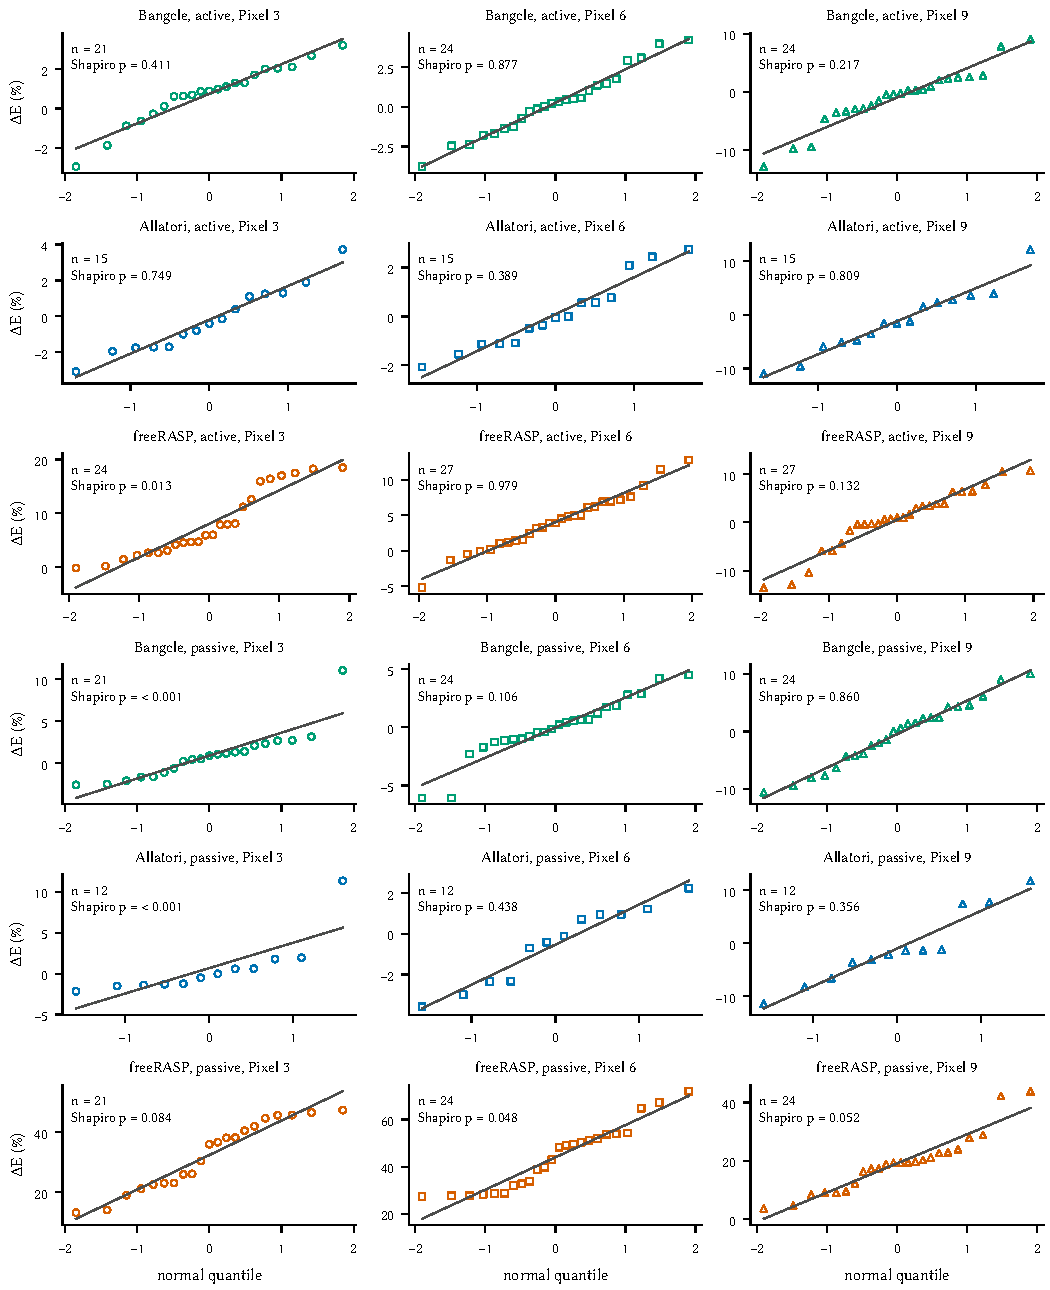
\includegraphics[width=\textwidth]{../figures/qq_per_device.pdf}
\caption{Q-Q plots of the paired differences for each technique, phase and device.}
\end{figure}
\FloatBarrier
\begin{figure}[p]
\centering
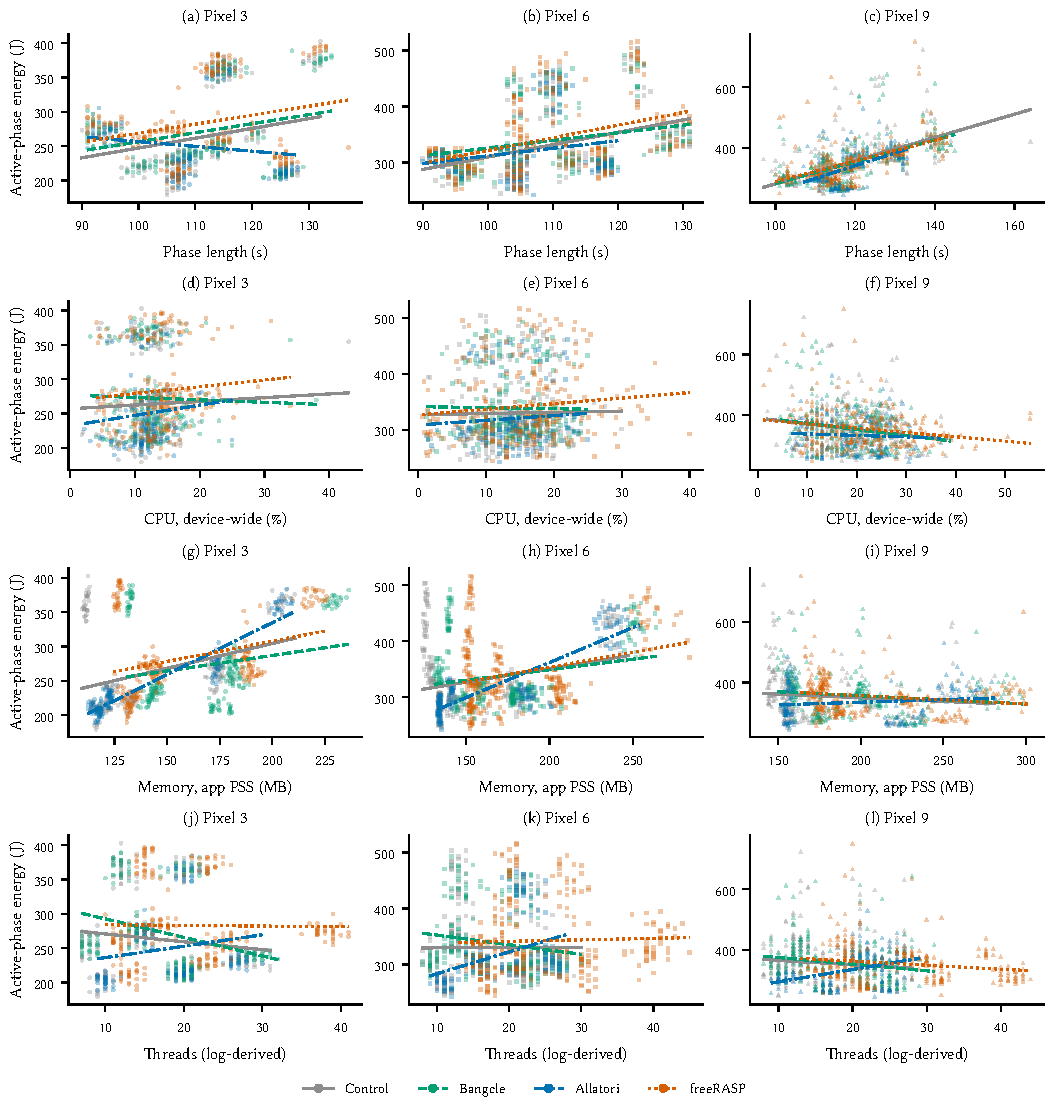
\includegraphics[width=\textwidth]{../figures/figure_rq3_active.pdf}
\caption{Active phase: energy per measurement against phase length, processor utilisation (device-wide), memory and thread count, per device; one point per measurement, a least-squares line per build.}
\end{figure}
\FloatBarrier
\begin{figure}[p]
\centering
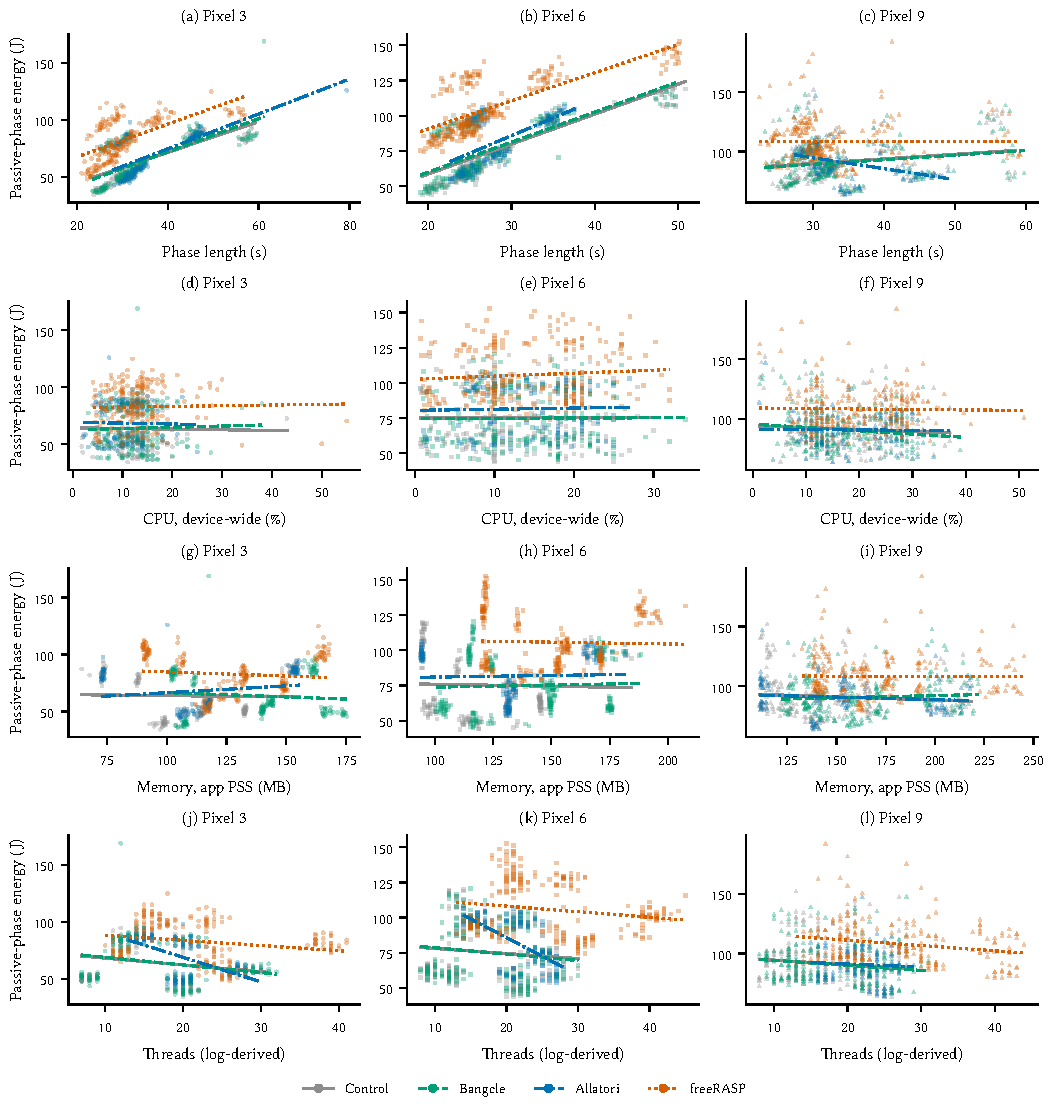
\includegraphics[width=\textwidth]{../figures/figure_rq3_passive.pdf}
\caption{Passive phase, as Figure S2; medtimer is not included.}
\end{figure}
\FloatBarrier
\end{document}
